
% % Load basic packages
% \usepackage{balance}       % to better equalize the last page
% \usepackage{graphics}      % for EPS, load graphicx instead 
% \usepackage[T1]{fontenc}   % for umlauts and other diaeresis
% \usepackage{txfonts}
% \usepackage{mathptmx}
% \usepackage[pdflang={en-US},pdftex]{hyperref}
% \usepackage{color}
% \usepackage{booktabs}
% \usepackage{textcomp}

% % Some optional stuff you might like/need.
% \usepackage{microtype}        % Improved Tracking and Kerning
% % \usepackage[all]{hypcap}    % Fixes bug in hyperref caption linking
% \usepackage{ccicons}          % Cite your images correctly!
% % \usepackage[utf8]{inputenc} % for a UTF8 editor only

% If you want to use todo notes, marginpars etc. during creation of
% your draft document, you have to enable the "chi_draft" option for
% the document class. To do this, change the very first line to:
% "\documentclass[chi_draft]{sigchi}". You can then place todo notes
% by using the "\todo{...}"  command. Make sure to disable the draft
% option again before submitting your final document.
% \usepackage{todonotes}
\chapter{ReMap: Multimodal Help-Seeking}
\label{chapter:remap}
\begin{quote}
People are reluctant to search for help when they feel it will take more time than trial-and-error exploration, even with a contextual search system like RePlay. However, trial-and-error often takes a long time or does not result in a correct solution. Given this cognitive bias, how might we lower the barrier to searching for help? This chapter aims to make searching easier and faster through multimodal interaction. We introduce \textit{ReMap}, an extension to the RePlay system that allows users to speak search queries, adding app-specific terms deictically. Users can navigate ReMap's search results via speech or mouse. A lab study showed that ReMap helped people stay focused on their task while simultaneously searching for and using help resources. Users' experiences with ReMap also raised a number of important challenges with incorporating multimodal features into a help-seeking system.
\end{quote}

\section{Introduction}
Despite the ubiquity of online search, help-seeking remains a tedious and difficult process for many. While the Web is ripe with knowledge and expert help, using it requires switching mental context, visual attention, and input focus away from the task at hand. As the RePlay study showed, these drawbacks often prevent people from searching altogether. Though bringing the search interface closer to the user's workflow and tying in relevant context seemed to help people spend less time once they decided to search, there was still an initial barrier that prevented many from searching in the first place. 
Coming up with an appropriate search query can be prohibitively difficult for novices, who may not know the correct vocabulary [dan russell]. It also switches the user's attention from the task at hand to the task of articulating their goal in a way that will match the resources they seek. How might we lower the barrier to searching and make it easier for people to find the resources they need in the moment?

When people help each other, they often use language, gestures, and context. Our research investigates how computers might do this too. The combination has allowed people of different backgrounds to communicate information and interact. Although it is a habit of humans to incorporate language, gestures, and context into assisting others, computers do not develop this knowledge unless programmed to. 

This chapter explores how multimodal interaction might make searching easier in the moment. Different types of information lend themselves better to different modalities; leveraging the strengths of multiple modalities and integrating them smoothly can be extremely effective \cite{Oviatt1999}. For example, combining speech and pointing allows people to communicate more precisely and efficiently by using deictic terms (\textit{e.g.,} ``this'', ``here'') to refer to objects and locations \cite{Bolt1980, Linder2013}. Furthermore, using multiple modalities simultaneously can improve efficiency; \textit{e.g.,} navigating tutorial videos with speech while one's hands are busy with a physical task \cite{Chang2019}. Finally, multimodal systems can also enable more natural interaction; \textit{e.g.,} letting users describe photo edits in their own words and inferring the appropriate commands \cite{Linder2013}, or activating software commands with speech rather than memorizing keyboard shortcuts \cite{Kim2019}.

\begin{figure}
\centering
  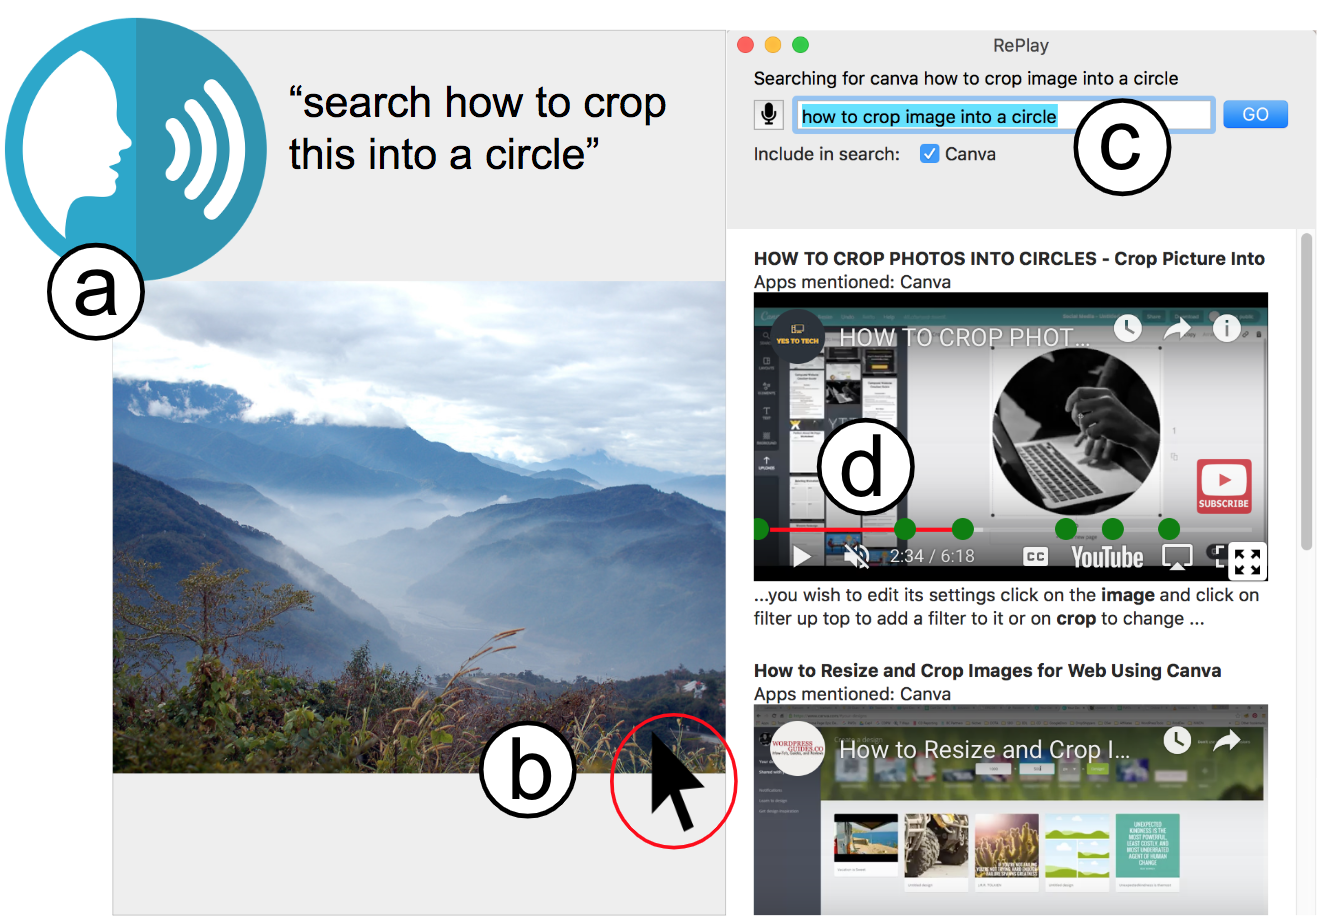
\includegraphics[width=\textwidth]{remap/figures/interface.png}
  \caption{ReMap is a multimodal search interface for finding learning videos. a) The user speaks their query. b) The user clicks on an image on the canvas while saying the word ``this.'' c) ReMap automatically changes the word ``this'' to ``image.'' d) ReMap highlights relevant moments by placing markers on the timeline of each video result.}~\label{fig:remap_interface}
  \vspace{-0.3in}
\end{figure}

We introduce ReMap, a multimodal interface for users to search for learning videos using speech and pointing, without taking their hands (or mouse) off their current task. ReMap builds on the existing video search interface RePlay \cite{Fraser2019}. ReMap's multimodal help search demonstrates three main design insights:
\begin{enumerate}
\item Users can initiate and dictate a search at anytime using speech, to avoid context-switching.
\item Users can point at elements in the software they are using to include their names in the search query, removing the need to remember app-specific terminology.
\item Users can play, pause, and navigate video results using speech, allowing them to simultaneously work on their task and follow along with a video tutorial.
\end{enumerate}

A study with 13 participants found that ReMap allows people to stay focused on their task while help-seeking. The study along with iterative prototyping and pilot testing also raised a number of important challenges with incorporating multimodal features into a help-seeking system.
\section{Related Work: Multimodal Interaction}
\subsection{The Power of Speech}
In 2016, Google reported that 20\% of all search queries on mobile Android devices were spoken \cite{Pichai2016}; that number has likely grown. Speech input is especially appealing on mobile devices, as people often use them while on the go and busy with other tasks \cite{Guy2016}, but even on desktop computers, voice assistants are often used for web search \cite{Mehrotra2016}. Speaking a search query is often easier and faster than typing it out, and it allows the user to ask a question like they might to a friend: mobile voice queries tend to be closer to natural language and more often phrased as questions than text queries \cite{Guy2016}. Also, people tend to search by voice more when seeking audio or video results \cite{Guy2016}, supporting ReMap's approach of using speech to search for videos. Finally, speech may be more useful for users with specific goals: Laput et al. \cite{Laput2013} found that when editing photos, speech was most useful when people knew exactly what they wanted to do. When people didn't know what they wanted, browsing a gallery of examples was more helpful as it allowed them to compare visual previews of potential effects before choosing one. Our studies with RePlay found that it was similarly most helpful for people with targeted questions, so we hypothesize that speech may be a useful way to search for help in ReMap.

\subsection{Combining Modalities can Maximize Cognitive Abilities}
Combining input from multiple modalities (\textit{e.g.}, speech, gesture, touch) can reduce cognitive load for complex tasks \cite{Oviatt2015, Reeves2004}, make tedious tasks more efficient \cite{Oviatt1999, Salisbury1990, Karl1993, Hugunin1997}, reduce errors \cite{Oviatt1999}, increase precision \cite{Cohen1989}, and even make tasks more enjoyable \cite{Oviatt1999, Laput2013}. Such combinations work best when they maximize users' working memory by using different modalities for different types of information \cite{Oviatt2015, Kalyuga1999, Reeves2004, Stanney2004}. 
%Auditory output is helpful for giving the user information while they work \cite{Stanney2004, Grossman2007, Reeves2004}, and visual output and manual input are helpful for conveying spatial information \cite{Stanney2004, Reeves2004}. 
For example, telling the user about keyboard shortcuts for the commands they execute via auditory feedback increases the likelihood that users will retain them, as users' auditory working memory is otherwise unused when working in software \cite{Grossman2007}. Similarly, using speech to navigate tutorial videos while one's hands are busy with a physical task allows users to process both the video and the task simultaneously \cite{Chang2019}. ReMap similarly partitions different modalities between the user's creative task and ReMap's help-seeking interface (\autoref{fig:remap_modalities}), allowing users to speak search queries and commands for navigating videos.

\begin{figure}[t]
\centering
  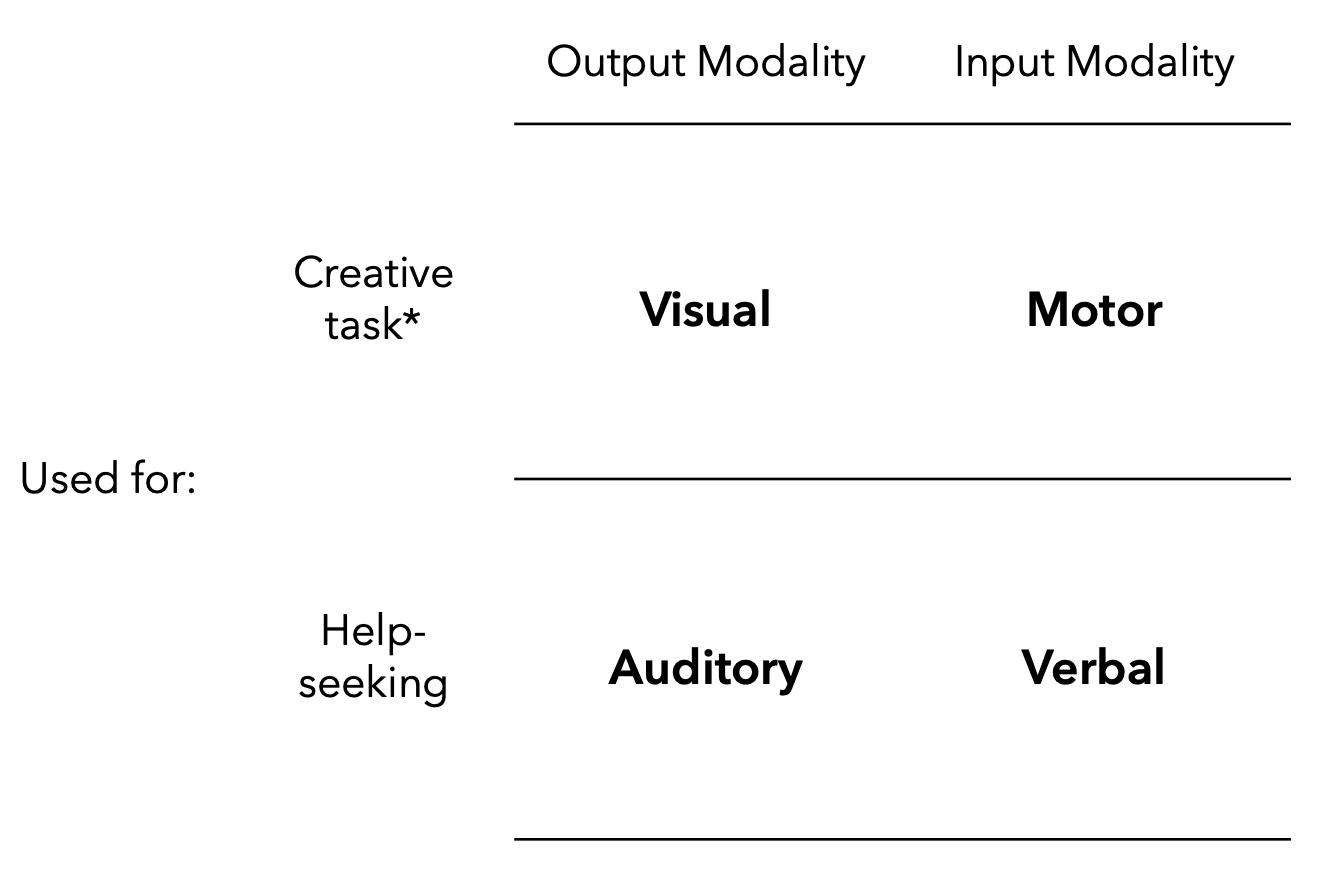
\includegraphics[width=0.7\textwidth]{remap/figures/remap_modalities.png}
  \caption[ReMap partitions the above modalities between the user's creative task and their help-seeking task to maximize cognitive abilities. Users primarily use speech and listening to search for and navigate help videos while keeping their hands and eyes on their creative task.]{ReMap partitions the above modalities between the user's creative task and their help-seeking task to maximize cognitive abilities. Users primarily use speech and listening to search for and navigate help videos while keeping their hands and eyes on their creative task. The * indicates that the visual and motor modalities are not \textit{exclusively} used for the creative task; users can also transfer their visual and motor attention to the help resources when necessary, \textit{e.g.}, to watch a video or type a search query manually.}~\label{fig:remap_modalities}
\end{figure}

Pointing at objects and spatial locations is often easier and more natural than describing them in words only \cite{Reeves2004, Bolt1980, Larkin1987}. Similarly, using a screenshot of an interface element as a search query is easier than describing it in text \cite{Yeh2009}. When combined with speech, pointing allows people to communicate more precisely by using deictic terms (\textit{e.g.,} ``this'', ``here'') to refer to objects and spatial locations while pointing at them \cite{Bolt1980, Laput2013}. ReMap similarly allows users to point at interface elements and canvas objects in their creative software and reference them deictically while speaking a search query.

Multimodal input can be especially beneficial for creative tasks, where maintaining a flow state is important. Using different modalities for software-related actions allows users to keep their focus and hands on their creative work. For example, using speech to access commands instead of menus or keyboard shortcuts can help artists maintain creative flow and stay focused on their task \cite{Kim2019, Sedivy1999}. While doing digital painting, an artist could switch from the brush tool to the eraser by saying ``eraser'' instead of switching their attention and moving their hands to the toolbar or keyboard \cite{Kim2019}. Not surprisingly, much prior work exploring multimodal input has centered around creative tasks such as photo editing \cite{Laput2013}, graphic design \cite{Kim2019}, drawing \cite{Sedivy1999, Pausch1991}, data visualization \cite{Setlur2016}, and 3D modeling \cite{Sharma2011}. However, most of this prior work has used speech to execute commands, rather than issue search queries. This requires either defining a list of acceptable commands (which users must then memorize) or parsing natural language commands (which is prone to errors). This chapter combines insights from multimodal creative systems and voice search systems to explore how voice search might be useful in creative software.

\section{ReMap System Design and Implementation}
ReMap (\autoref{fig:remap_interface}) extends the RePlay contextual search system \cite{Fraser2019}. RePlay enables users to search for learning videos in context while working in software, and it highlights relevant moments in video results based on the user's context and query. While RePlay helps people find results faster, the attentional cost of switching to RePlay discouraged its being used as often as it could. ReMap lowers the switching cost and load by introducing three main improvements over RePlay: searching for help using speech, making deictic references in a search query, and navigating video results using speech commands.

\subsection{Searching for help using speech}
ReMap uses the Web Speech \textsc{api} to detect speech by opening a browser page in the background when launched. This page can be minimized or hidden by the user. The first time it opens it asks the user to grant access to the microphone; all subsequent uses will grant access automatically. The page's JavaScript invokes continuous listening and sends the current phrase to ReMap's custom web server whenever a new word is detected.
The Web Speech \textsc{api} automatically determines when the user starts and finishes speaking, returning each phrase separately. If a phrase begins with the word \textit{``search''}, ReMap initiates a search (\autoref{fig:remap_interface}a), using the rest of the phrase as the query. Otherwise, it checks if the phrase matches any video navigation commands. If it does not, ReMap ignores it.

\subsection{Making deictic references in a search query}
Especially with new software, people are often unfamiliar with an application's vocabulary but can point at application elements that are relevant to their goal. 
To alleviate the challenge of remembering app-specific terms, ReMap allows users to deictically reference interface elements and objects while speaking their query. If the user says \textit{``this''} or \textit{``that''} while clicking on a detectable element, ReMap replaces the pronoun with the reference element's name (\autoref{fig:remap_interface}b-c). Like RePlay, ReMap uses the MacOS Accessibility \textsc{api} to resolve element names. 
%This \textsc{api} can get the name and description of any element with accessibility labels \cite{Fraser2019}. Many modern applications have labeled menus, buttons, and other interface elements. Some also label canvas elements (such as text boxes, images, and graphics) though many do not. The examples in this demo use Canva (\url{canva.com}) as the primary software. Canva labels most canvas elements and interface buttons.

While ReMap is detecting a speech query, it stores a list of every detectable element clicked. Once the user is finished speaking and ReMap has obtained the final query from the server, it replaces all occurrences of \textit{``this''} and \textit{``that''} with the element names in the order they were clicked before issuing the search query.

\begin{figure}[b!]
\centering
  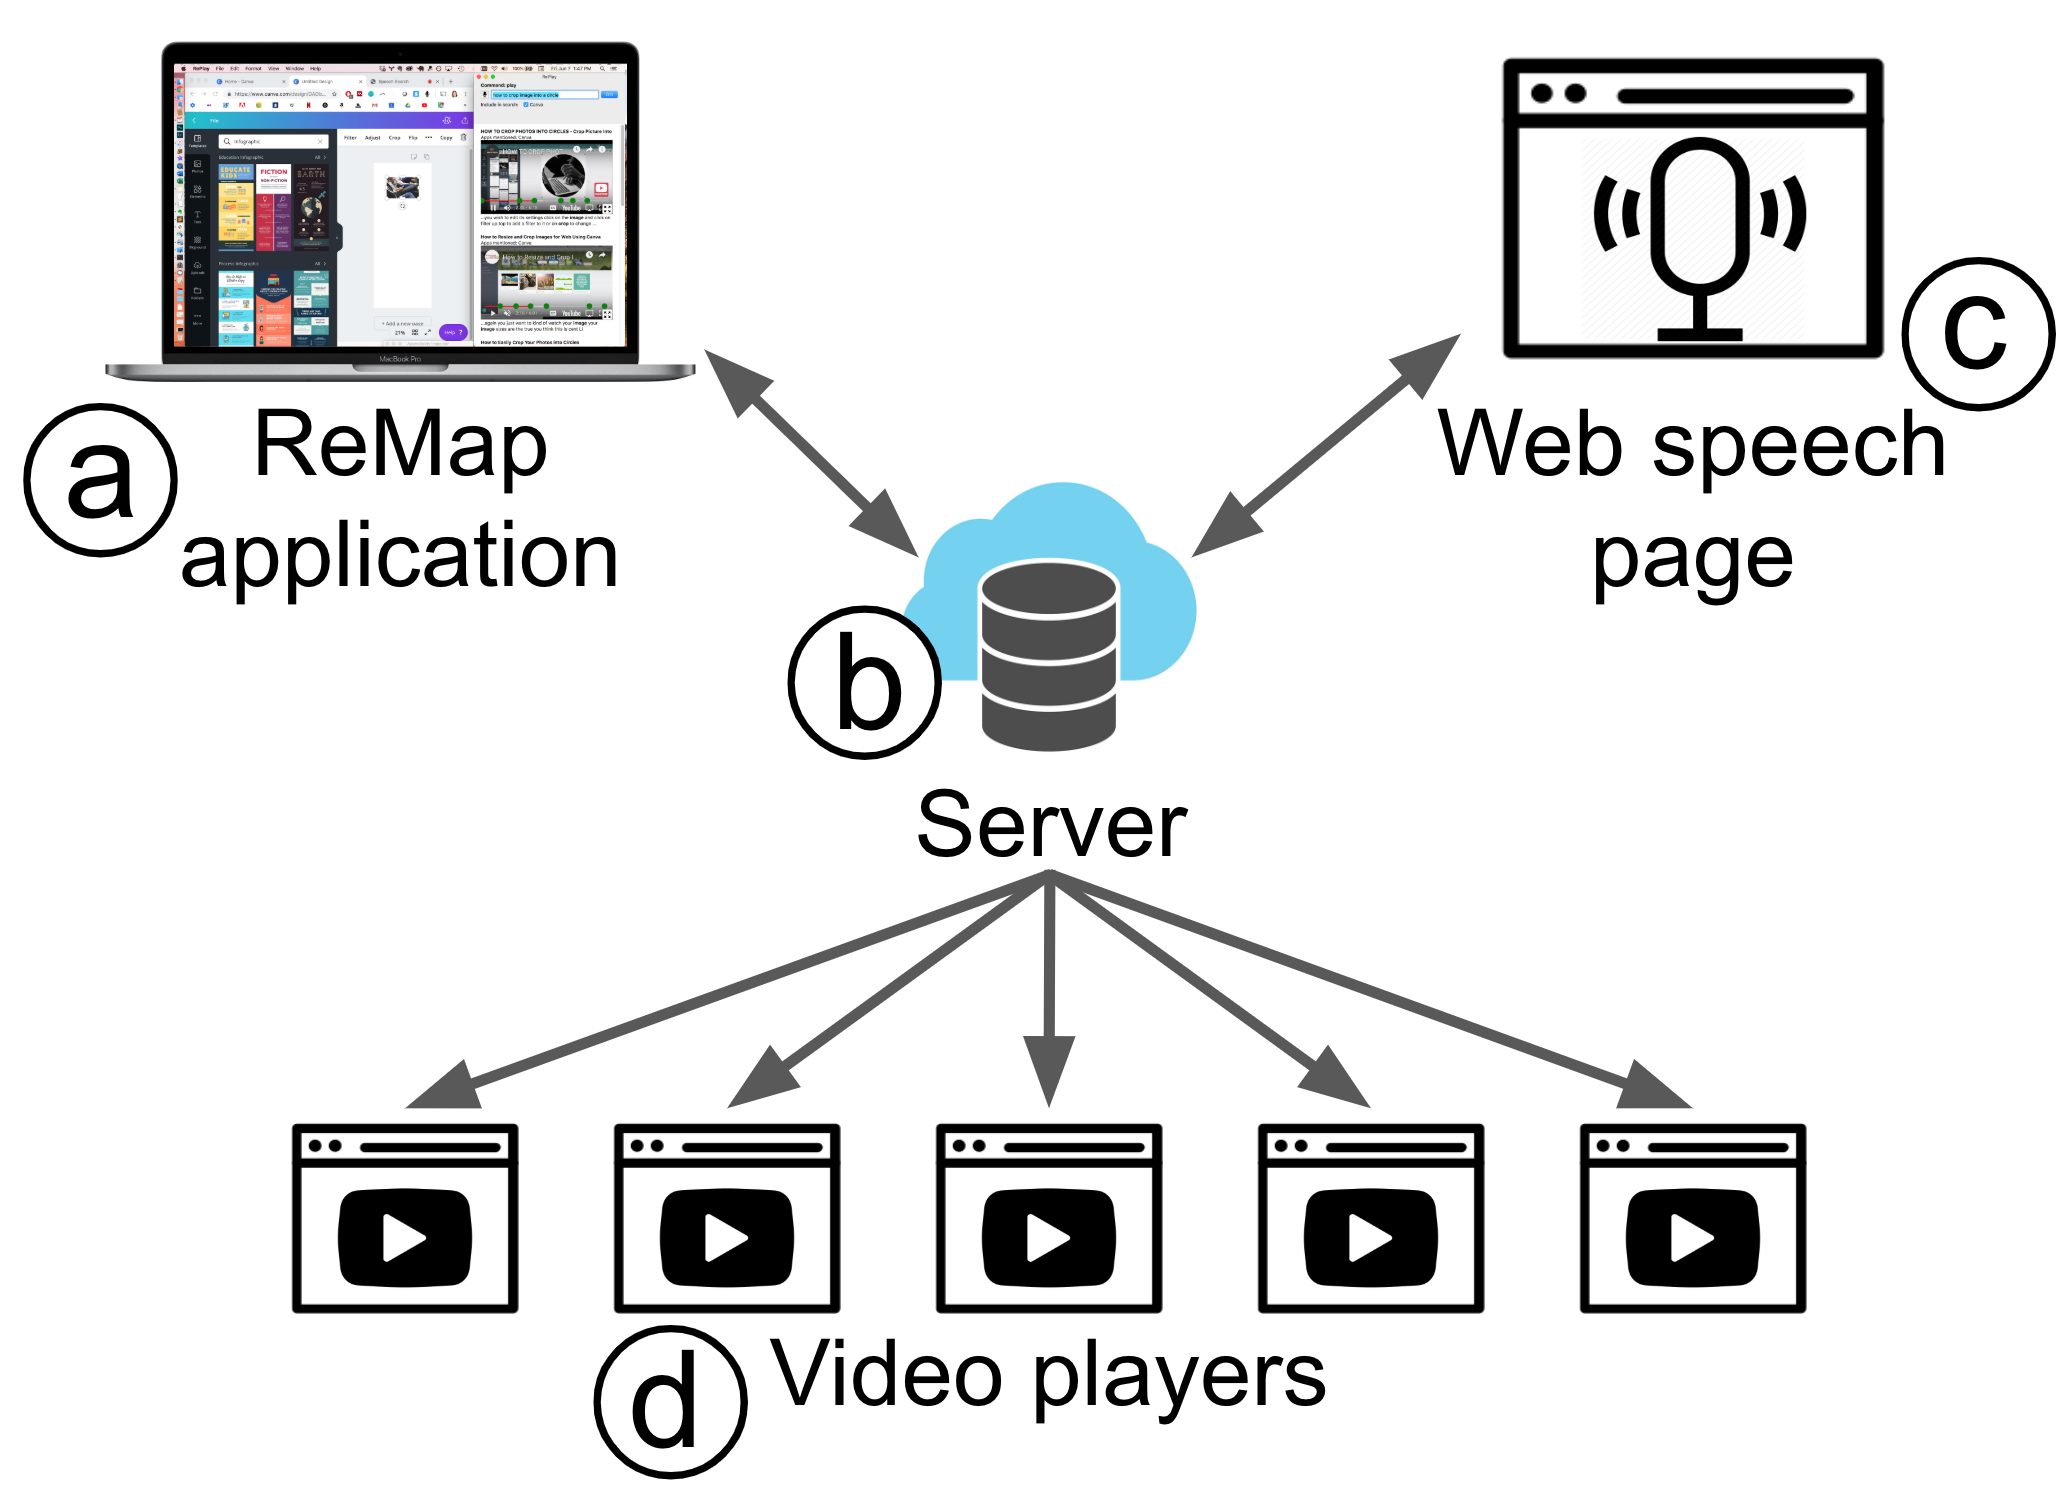
\includegraphics[width=\textwidth]{remap/figures/system.png}
  \caption{The ReMap system architecture. a) ReMap is a MacOS application that uses the Accessibility \textsc{api} to detect user context. b) ReMap connects to a web server, which opens c) a webpage for speech recognition, and d) a video player webpage for each result to embed in ReMap.}~\label{fig:remap_system}
  \vspace{-0.2in}
\end{figure}

\subsection{Navigating video results using speech commands}
The user can speak commands to navigate video results, inspired by Chang \textit{et al.}'s recommendations \cite{Chang2019}. ReMap currently supports the following commands: \textit{``play''} (plays the first or most-recently played video), \textit{``play \{next, previous, last\}''} (plays the next/previous/last video in the list), \textit{``play \{first, second, third, fourth, fifth\} video''}, \textit{``\{next, previous, repeat\} marker''} (skips to the next or previous timeline marker, or re-starts from the current marker), and \textit{``pause''} / \textit{``stop''} (pauses the currently playing video).


\subsection{Implementation}
ReMap is implemented as a MacOS Swift application (\autoref{fig:remap_system}a). It uses socket.io to communicate between the web server and the three client interfaces (the ReMap desktop application, web speech page, and video players). The web server (\autoref{fig:remap_system}b) is implemented in Node.js. The speech engine (\autoref{fig:remap_system}c) uses the Web Speech \textsc{api}, and the video player (\autoref{fig:remap_system}d) uses the YouTube Player \textsc{api} to load and control videos. ReMap generates a unique anonymous user ID for each computer it runs on. When it opens the speech engine and video player webpages, it includes this user ID as a parameter. For video player pages, it also includes that video's index in the result list. The server keeps track of these values for each client page that opens a socket connection, so that it can pass commands it receives to the appropriate client.

The web speech page determines whether a spoken phrase starts with the word \textit{``search''} and if so, sends the rest of the phrase to the server which sends it to the ReMap app as a query. If a phrase matches a video navigation command, the server sends this command to the ReMap app which then determines which video index it applies to, and returns a message to the server telling it which video player to send the command to. If the command was to play a different video than the currently playing video, ReMap also asks the server to pause the currently playing video.

\section{Study: Using ReMap for a Graphic Design Task}
\label{sec:remap_study}
To gain an initial understanding of how people use multimodal search for help, we conducted a think-aloud lab study with thirteen participants. Participants re-created a given design in Canva (\href{https://canva.com}{\nolinkurl{canva.com}}) and used ReMap to search for help when necessary. Overall we found that despite some usability and implementation challenges, multimodal video search was helpful, allowing participants to stay focused on their task while simultaneously searching for help and navigating video resources. 

\subsection{Participants}
Thirteen participants were recruited from mailing lists and flyers at a university. 10/13 participants had at least some experience using voice assistants (\textit{e.g.}, Siri, Amazon echo) (mean = 2.3/5, 1 = never used, 5 = use every day). 6/15 participants had never used Canva before, and only one was very familiar with it (mean = 1.8/5, 1 = never used, 5 = very familiar).

\subsection{Procedure}
Participants were shown two images of an infographic design (\autoref{fig:remap_designs}) and were asked to choose one and re-create it as accurately as possible in Canva without using any of Canva's built-in templates. Participants were asked to use ReMap only (no web search) when they needed to search for help. Participants were given a brief tutorial on how to use ReMap, and were given three example commands to try to ensure they understood how it worked. They were encouraged to use speech as much as possible, but also had the option to type their search queries into ReMap's search field. Participants were asked to think out loud while they worked, and the experimenters captured audio and screen recordings. Participants were scheduled for 2-hour slots and were told to take as much time as they needed. Once they announced they were done (or if 1 hour and 45 minutes had passed), participants were asked a series of interview questions including prompts for Likert-scale responses to understand how they felt the task went, and whether they found ReMap helpful. Participants received a \$30 USD gift card for their time.

\begin{figure}[t!]
\centering
  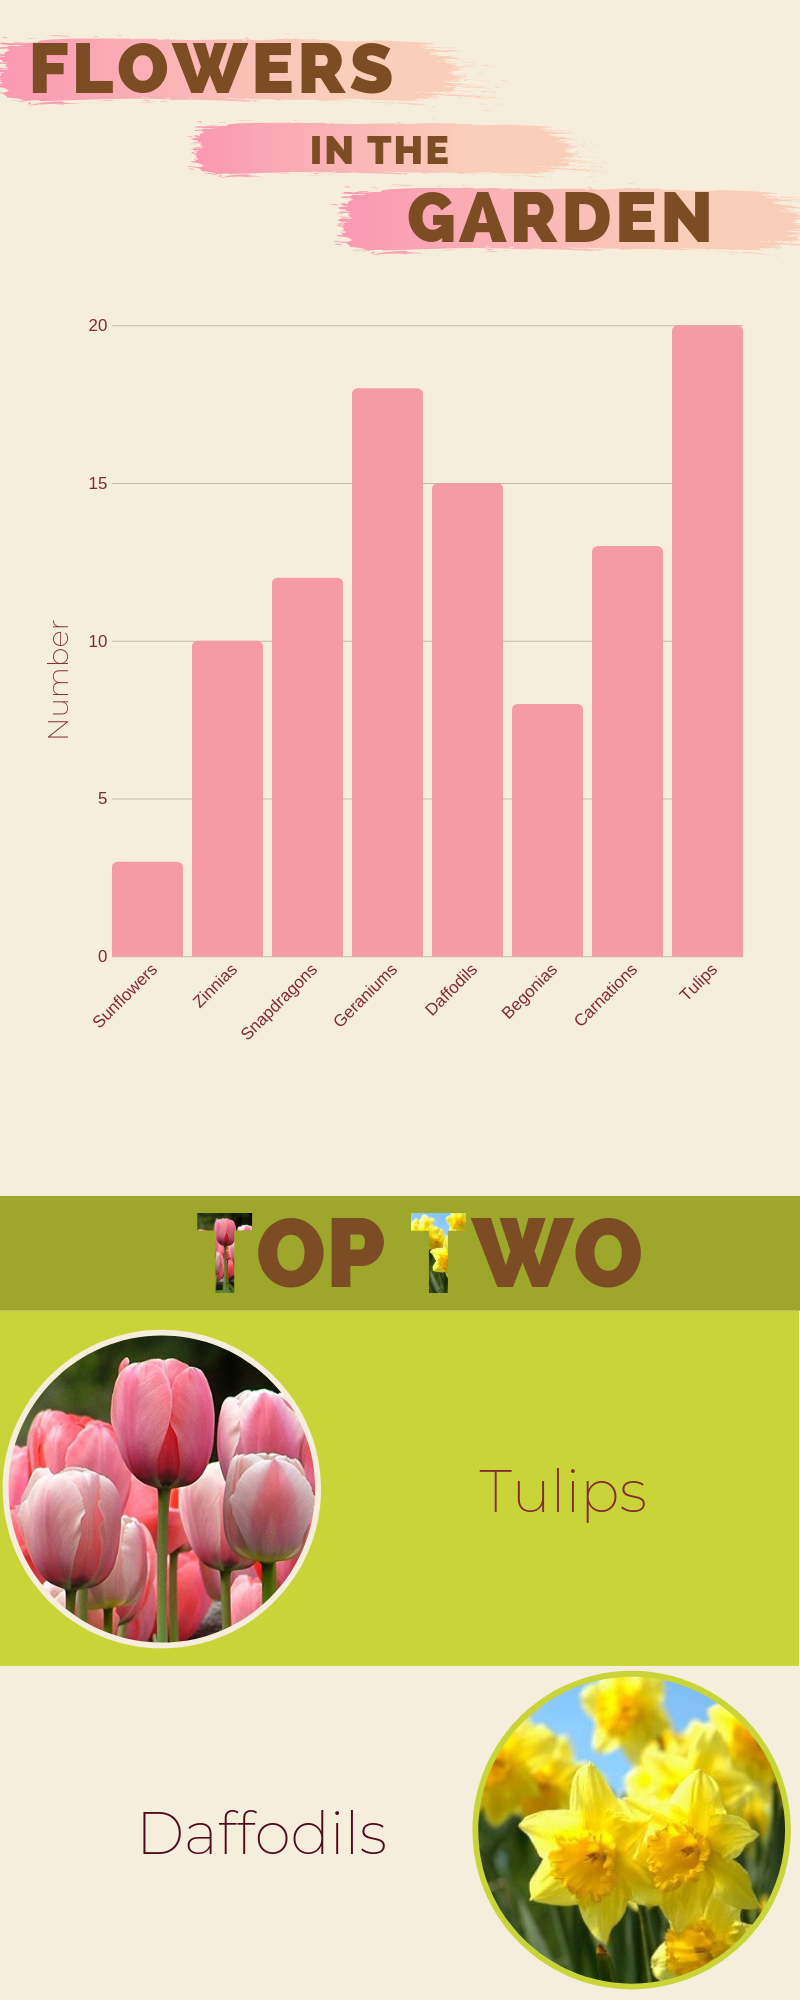
\includegraphics[width=0.3\textwidth]{remap/figures/designA.png}
  \hspace{0.2in}
  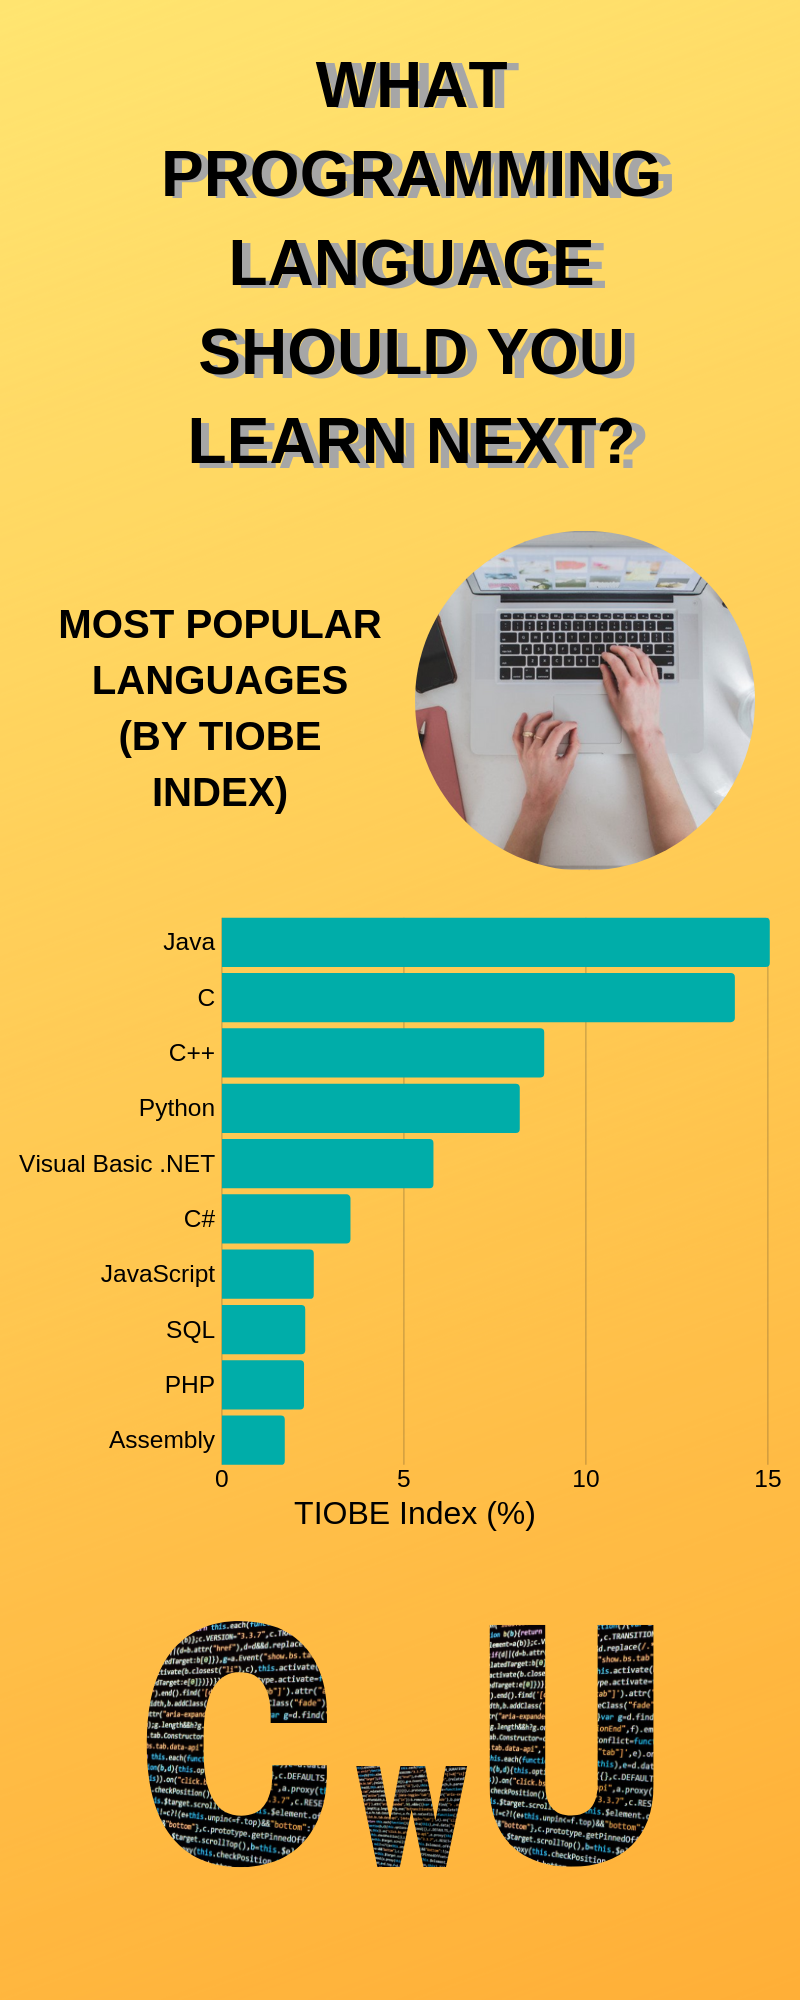
\includegraphics[width=0.3\textwidth]{remap/figures/designB.png}
  \caption{Study participants chose one of the above two infographic designs to re-create in Canva, using ReMap to search for help.}~\label{fig:remap_designs}
\end{figure}

Both infographics were designed to require several operations that are not straightforward in Canva, to increase the likelihood that participants would have to search for help. These included: cropping an image in a circle, masking an image in text, creating a bar chart given a spreadsheet of data, making a swish shape behind text (\autoref{fig:remap_designs} left only) and adding a shadow to text (\autoref{fig:remap_designs} right only).

ReMap's speech recognition requires a clear signal of the user's speech, mostly free of interference from sound output (\textit{i.e.} from videos) or background conversations. We have found commodity headsets to be sufficient, high-quality headsets to be optimal, and built-in laptop microphones insufficient. For the study, participants wore a high-quality headset.

\subsection{Results}
\subsubsection{Search Behaviour}
Participants issued a total of 118 intentional search queries, 111 of which used speech (\autoref{table:remap_results}). An additional 3 queries were issued by mistake (not realizing they had spoken the ``search'' command) and an additional 7 were issued before the participant had finished speaking (because the Web Speech \textsc{api} detected a pause). One participant did not search at all (the same participant that rated their familiarity with Canva as 5/5); the rest issued between 4 and 18 queries each. 

\begin{table}[b!]
\centering
\caption{Summary of each participant’s usage of ReMap. ``\# speech commands'' includes all play, pause, and marker navigation commands. ``\# manual commands'' includes all plays, pauses, seeking along the timeline, and clicking on markers.}~\label{table:remap_results}
\resizebox{1\textwidth}{!}{
\begin{tabular}{lllllllll}
\textbf{} & \textbf{\begin{tabular}[c]{@{}l@{}}Total \#\\ intentional\\ searches\end{tabular}} & \textbf{\begin{tabular}[c]{@{}l@{}}\# accidental or\\ pre-emptive\\ searches\end{tabular}} & \textbf{\begin{tabular}[c]{@{}l@{}}\# intentional\\ speech\\ searches\end{tabular}} & \textbf{\begin{tabular}[c]{@{}l@{}}\# unique\\ videos\\ played\end{tabular}} & \textbf{\begin{tabular}[c]{@{}l@{}}\# speech\\ commands\end{tabular}} & \textbf{\begin{tabular}[c]{@{}l@{}}\# manual\\ commands\end{tabular}} & \textbf{\begin{tabular}[c]{@{}l@{}}\# deictic\\ references\end{tabular}} & \textbf{\begin{tabular}[c]{@{}l@{}}\# successful\\ deictic\\ resolutions\end{tabular}} \\ \hline
P1 & 17 & 1 & 17 & 13 & 41 & 3 & 5 & 1 \\
P2 & 5 & 0 & 5 & 6 & 2 & 93 & 1 & 0 \\
P3 & 13 & 3 & 13 & 7 & 20 & 23 & 10 & 1 \\
P4 & 4 & 0 & 4 & 5 & 14 & 19 & 0 & 0 \\
P5 & 0 & 0 & 0 & 0 & 0 & 0 & 0 & 0 \\
P6 & 8 & 1 & 8 & 5 & 17 & 2 & 0 & 0 \\
P7 & 7 & 1 & 7 & 6 & 24 & 10 & 0 & 0 \\
P8 & 3 & 1 & 3 & 2 & 4 & 1 & 0 & 0 \\
P9 & 8 & 1 & 6 & 6 & 0 & 49 & 0 & 0 \\
P10 & 16 & 0 & 13 & 5 & 10 & 5 & 3 & 0 \\
P11 & 10 & 1 & 10 & 11 & 9 & 51 & 1 & 1 \\
P12 & 11 & 0 & 11 & 4 & 8 & 16 & 1 & 1 \\
P13 & 16 & 1 & 14 & 7 & 18 & 0 & 3 & 2 \\
\textbf{Total} & \textbf{118} & \textbf{10} & \textbf{111} & \textbf{77} & \textbf{167} & \textbf{272} & \textbf{24} & \textbf{6}
\end{tabular}
}
\end{table}

61/118 queries (52\%) were new queries and 34/118 (29\%) were reformulations of previous queries (i.e., rephrasing a query to find better results). The rest were either attempts to fix a failed deictic resolution or fixing a transcription error. 55/118 queries began with either the phrase ``how to'' (42/118), or the phrase ``how do I'' (13/118). 

8/111 speech queries included a speech recognition error. One participant tried to rephrase their query after speaking it twice, leading to long queries with some repetition (\textit{e.g.}, ``resize this without aspect ratio without keeping aspect ratio''). 6 of the 7 non-speech queries were a manual revision of a previous speech query (either error fixes or reformulations). 

7 of 13 participants used deictic references at least once. Only 6 of 24 total deictic references were successfully resolved to a name, mainly because some canvas objects were not recognizable by ReMap (\textit{e.g.,} graphs). 23/24 deictic references referred to objects on the canvas (\textit{e.g.}, text boxes, images, and graphs); the other one referred to a button on the toolbar. This reinforces RePlay's study finding (\autoref{sec:replay_study}) that participants mostly made action-oriented queries, rather than queries about tools or commands, and highlights the need for canvas elements to be recognizable by ReMap.

\subsubsection{Video Navigation Behaviour}
Participants watched a total of 77 videos (\textasciitilde6 videos per participant). In total, participants played videos by clicking on them 60 times, and by saying one of the ``play'' commands 61 times. Participants paused manually 60 times, and via the ``pause'' speech command 46 times. Participants manually seeked to points in the video by dragging on the timeline 124 times, by clicking timeline markers 28 times, and by using the ``next/previous/repeat marker'' commands 60 times. In general, most participants seemed to exhibit a preference for either speech commands or manual navigation of videos (\autoref{table:remap_results}). This highlights the importance of providing both options in a multimodal interface, especially as peoples' preferences and needs may change depending on their task or environment \cite{Reeves2004, LaViolaJr.2014}.

\subsubsection{Participant Feedback}
As \autoref{fig:remap_boxplot} shows, participants generally found all four of ReMap's multimodal features moderately helpful. Based on our observations, most participants used the multimodal features to work and search or watch videos simultaneously. They confirmed this during the post-task interviews, with several participants explicitly mentioning multitasking as a benefit of ReMap's multimodal features. For example, one participant described how ReMap helped them be more efficient than their current strategies for help-seeking:

\begin{quote}
\textit{``When I'm designing graphics myself sometimes I get stuck, so I will have to stop everything and go to YouTube or Google to find it, but if I'm able to work while listening or ... watching it on the side, through voice, I think it will help with efficiency ... `cause at one point I was able to ... move the things around while listening for the things I need.''} --- P4
\end{quote}

\begin{figure}[t!]
\centering
  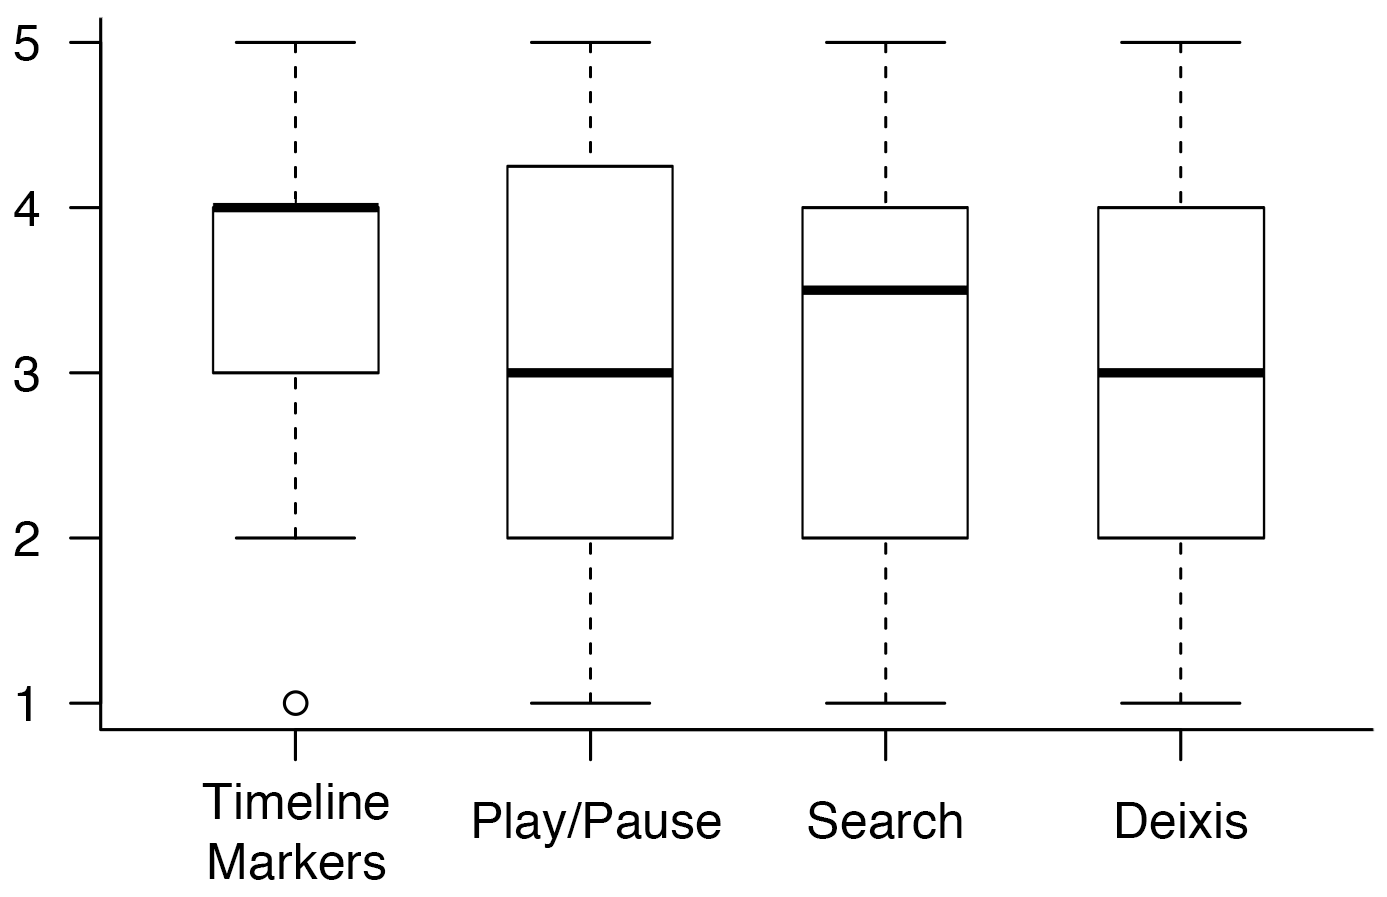
\includegraphics[width=0.7\textwidth]{remap/figures/boxplot.png}
  \caption{Distribution of participants' ratings of ReMap’s multimodal features. 1 = not helpful at all, 5 = very helpful. Bold lines represent median values, and boxes illustrate interquartile ranges. }~\label{fig:remap_boxplot}
\end{figure}

\textbf{Timeline markers:}
Navigating the timeline markers was rated as the most helpful multimodal feature on average, and was the most common answer participants gave when asked what their favorite feature of ReMap was. This is mainly because it supported participants in multitasking:

\begin{quote}
\textit{``I ... found it helpful because while it was switching I could multitask, and I could just tell it `hey, go to the next marker', and then I would try to do stuff on my own on the side until it plays.''} --- P6
\end{quote}

\begin{quote}
\textit{``If I couldn't use speech then i would have to ... actually click on the videos, but since I'm already working on this part of the screen, then [speech is] just more convenient.''} --- P7
\end{quote}

The markers themselves were useful (as the RePlay study (\autoref{sec:replay_study}) also showed) as they provided a shortcut to potentially relevant moments in the video. The speech commands for skipping between them made it easy for participants to back-up or fast-forward the video to a reasonable point. This is easier than having to specify a specific time interval to skip between, which Chang et al. \cite{Chang2019} showed can be difficult for people following along with video tutorials. However, some participants did mention that they preferred using the mouse to hover over markers before selecting them, so they could see the caption previews (\autoref{fig:replay-green_markers}): \textit{``I don't really know what they are until I scroll over them''} (P11).

\textbf{Play/pause:}
Some participants also found speech for playing and pausing videos to be helpful, as it allowed them to follow along with videos at their own pace, which prior work has also demonstrated the importance of \cite{Chang2019, Pongnumkul2011}.

\begin{quote}
\textit{``It's really helpful because if I hear the info I want and I'm kind of following along I can pause it, take the instructions, apply it, and then ... continue watching ... without having to stop the fluidity of work.''} --- P8
\end{quote}
\begin{quote}
\textit{``It was nice to be able to keep track of the video in the background while also starting to think through the next thing and having my focus on the other window.''} --- P13
\end{quote}

Other participants preferred using the mouse to play and pause the videos as they felt it was just as fast or easy, and didn't require them to remember the correct wording of the commands.

\textbf{Speaking query:}
Many participants found it helpful to speak their query out loud rather than type it, as it also supported multitasking and allowed them to stay focused on the task in Canva. Some also said that it was easier or faster than typing. However, some other participants found it more difficult to speak their query, as they didn't always know exactly what to say when they started, and they were not used to speaking out loud to search. As P13 described, \textit{``I had a lot of trouble getting my queries totally straight or thought out in my head before starting to speak them.''} One common difficulty encountered with ReMap's implementation was that it would cut off a participant's query and issue the search before they were done speaking, often because they paused slightly while thinking of what to say. This happened 7 times and was due to the Web Speech \textsc{api} prematurely detecting the end of a phrase. As one participant described, it made them feel rushed to finish speaking:

\begin{quote}
\textit{``It kept rushing me to think about what I wanted to search for ... Usually when I search by typing, I type out half of what I want and then think about ... what to type for the rest, whereas here as soon as i said `how to add' I had to immediately know what I was searching.''} --- P6
\end{quote}

\textbf{Deixis:}
The 7 participants who attempted using deixis in their queries mostly found it helpful, although many noted that it needed some improvement to be useful. It helped participants include words they didn't know in their queries and was often easier and faster than saying or typing the words explicitly. However, it is likely most helpful in cases where users do not know the terminology, and Canva's interface has a relatively straightforward vocabulary. For example, P1, who rated their prior experience with Canva as 1.75/5, said \textit{``it might be more helpful for things that you don't know the exact terminology for, but I think I knew some of the terminology so just saying it felt faster.''}

ReMap's deictic resolution also suffered some implementation and usability challenges: deictic references were only successfully resolved 25\% of the time, usually due to objects on the canvas not being recognized by the Accessibility \textsc{api}. Two participants also pointed out that their eyes naturally went to the search field where their query was appearing while they spoke it, which made it difficult to look at Canva instead to reference elements: \textit{``even though i was trying to click here i was focusing on [the search field]''} (P9).

\textbf{Overall:}
Finally, when asked if participants could see themselves using ReMap in their daily lives, 9 participants said yes (3 saying for certain tasks only, and 2 saying if the technology improved first). The 4 participants who said no shared reservations about using speech in public or around people, and some said they simply prefer typing.

\section{Discussion / Challenges}
\subsection{Implementation Challenges}
- having to be a macos app because accessibility, but no good speech so having to use web speech api
- accessibility in general not super good --> deictic failed a lot
\subsection{Usability Challenges}
- searching unintentionally (midas touch)
- or not listening when keyword was misheard
- cutting off before they were done talking
- correcting query is hard, mostly resort to typing or people would repeat themselves but system isn't that smart
- showing query as they spoke might have been distracting - they weren't looking at the task anymore
\subsection{Potentail IMprovements / future exploration to do}
- compare keyword to search vs. button / keyboard shortcut
- let user decide when done talking (adds extra step but could prevent errors)
- explore how to correct queries (existing work?) using speech -- detect if they repeat themselves and go with the second version, or suport things like "x instead of y"
- compare not showing query (just listening) vs. showing it
- other ways to do deictic -- computer vision like prefab?
- higher level -- do people really want deictic? is it useful? most queries (as we found with replay too) were not about tools so being able to refer to them isn't that useful, and other things (like objects on the canvas) people mostly know what they are called so it doesn't save much time
- deictic may be more useful for issuing commands or sending questions to people / posting in forums
\section{Conclusion}
ReMap introduces multimodal interaction for quick, in-context help-seeking by leveraging the strengths of multiple modalities. Users can search for videos using speech, use deixis to include application-specific terminology, and use speech to navigate videos. An initial study showed that ReMap helps people stay focused on their task while navigating help resources, and highlighted several important challenges with multimodal search. 
%Future work should explore how to make deictic resolution more robust and further lower the barrier to searching in context.

RePlay and ReMap demonstrated how bringing learning videos into the user's context can help people find procedural help while working toward a specific desired outcome. The next chapters in this dissertation break apart the goals of \textit{process} and \textit{outcome}, exploring how contextual systems can support users who desire only one or the other.

\section{Acknowledgements}
This chapter, in part, is currently being prepared for submission for publication of the material. C. Ailie Fraser, Julia M. Markel, N. James Basa, Mira Dontcheva, and Scott Klemmer. The dissertation author was the primary investigator and author of this material.

